\documentclass[12pt]{report}
\usepackage{graphicx}
\usepackage{amsmath}
\usepackage{fancyhdr}
\usepackage{geometry}
\usepackage{circuitikz}
\usepackage{subfigure}
\usepackage{caption}
\usepackage{karnaugh-map}
\usepackage{bm}

\geometry{letterpaper, margin=1in}
\graphicspath{ {../images/} }

% Header and Footer
\pagestyle{fancy}
\fancyhf{}
\fancyhead[L]{CSE 2301 - Lab 03: I/O and POSTNET}
\fancyhead[R]{\thepage}
\setlength{\headheight}{15pt}

\author{Arturo Salinas-Aguayo}
\title{Lab 03: I/O and POSTNET3: I/O and POSTNET3: I/O and POSTNET}
% theorem set
\newtheorem{example}{Example}
% Example block environment
\newenvironment{examp}
{\vspace{0.5cm}
\hrule
\begin{example}}
{\hrule
\vspace{0.5cm}
\end{example}}

\begin{document}
\newcommand{\closure}[2][3]{%
	{}\mkern#1mu\overline{\mkern-#1mu#2}}
\newcommand\ncoverline[1]{\mkern1mu\overline{\mkern-1mu#1\mkern-1mu}\mkern1mu}
% Title Page
\begin{titlepage}
	\centering
	\vspace*{3cm}
	\huge\textbf{Lab 03: I/O and POSTNET}\\
	\vspace{5cm}
	\Large\textbf{Arturo Salinas-Aguayo}\\
	\normalsize
	CSE 2301: Principles and Practice of Digital Logic Design\\
	Dr. Mohammad Khan, Section 003L-1248\\
	Electrical and Computer Engineering Department
	\vfill
	
\includegraphics[scale=0.1]{uconnlogo}\\
	College of Engineering, University of Connecticut\\
	\scriptsize{Coded in \LaTeX}
	\vspace*{1cm}
\end{titlepage}
\section*{Theory}
\subsection*{The 7405 Chip DIP}
The \textbf{7405 DIP} \textit{(Dual-Inline-Package)} from Texas Instruments is a different kind of inverter called an \textit{Open Collector}, compared to the \textbf{7404 DIP} by the same manufacturer which is a standard inverter with something called a \textit{Push-Pull Output Stage.} Our application requires driving a load, in this case some Light Emitting Diodes. These LEDs require higher current draw which a \textbf{7404} IC cannot handle directly. The \textbf{7405} provides the ability to drive an external load by pulling the output signal to ground without having to supply or drive the current from the IC itself.

\subsubsection*{The Bipolar Junction Transistor}
In order to properly explain this choice, the \textit{emitter, base,} and \textit{collector} of a Bipolar Junction Transistor must be properly defined.
\begin{examp}
	\textbf{The Bipolar Junction Transistor Abstraction}
	\newline
	\textbf{Emitter}
	\textnormal{A \textit{heavily} doped, medium-sized layer designated to inject or emit electrons.}
	\newline
	\textbf{Base}
	\textnormal{A thin layer of \textit{medium} doped material designed for electron transmission.}
	\newline
	\textbf{Collector}
	\textnormal{A wide layer of \textit{lightly} doped material designed to \textit{collect} electrons.}
	\newline
	Texas Instruments utilizes NPN Transistors in their schematics such as this:
	\begin{figure}[h]
		\center{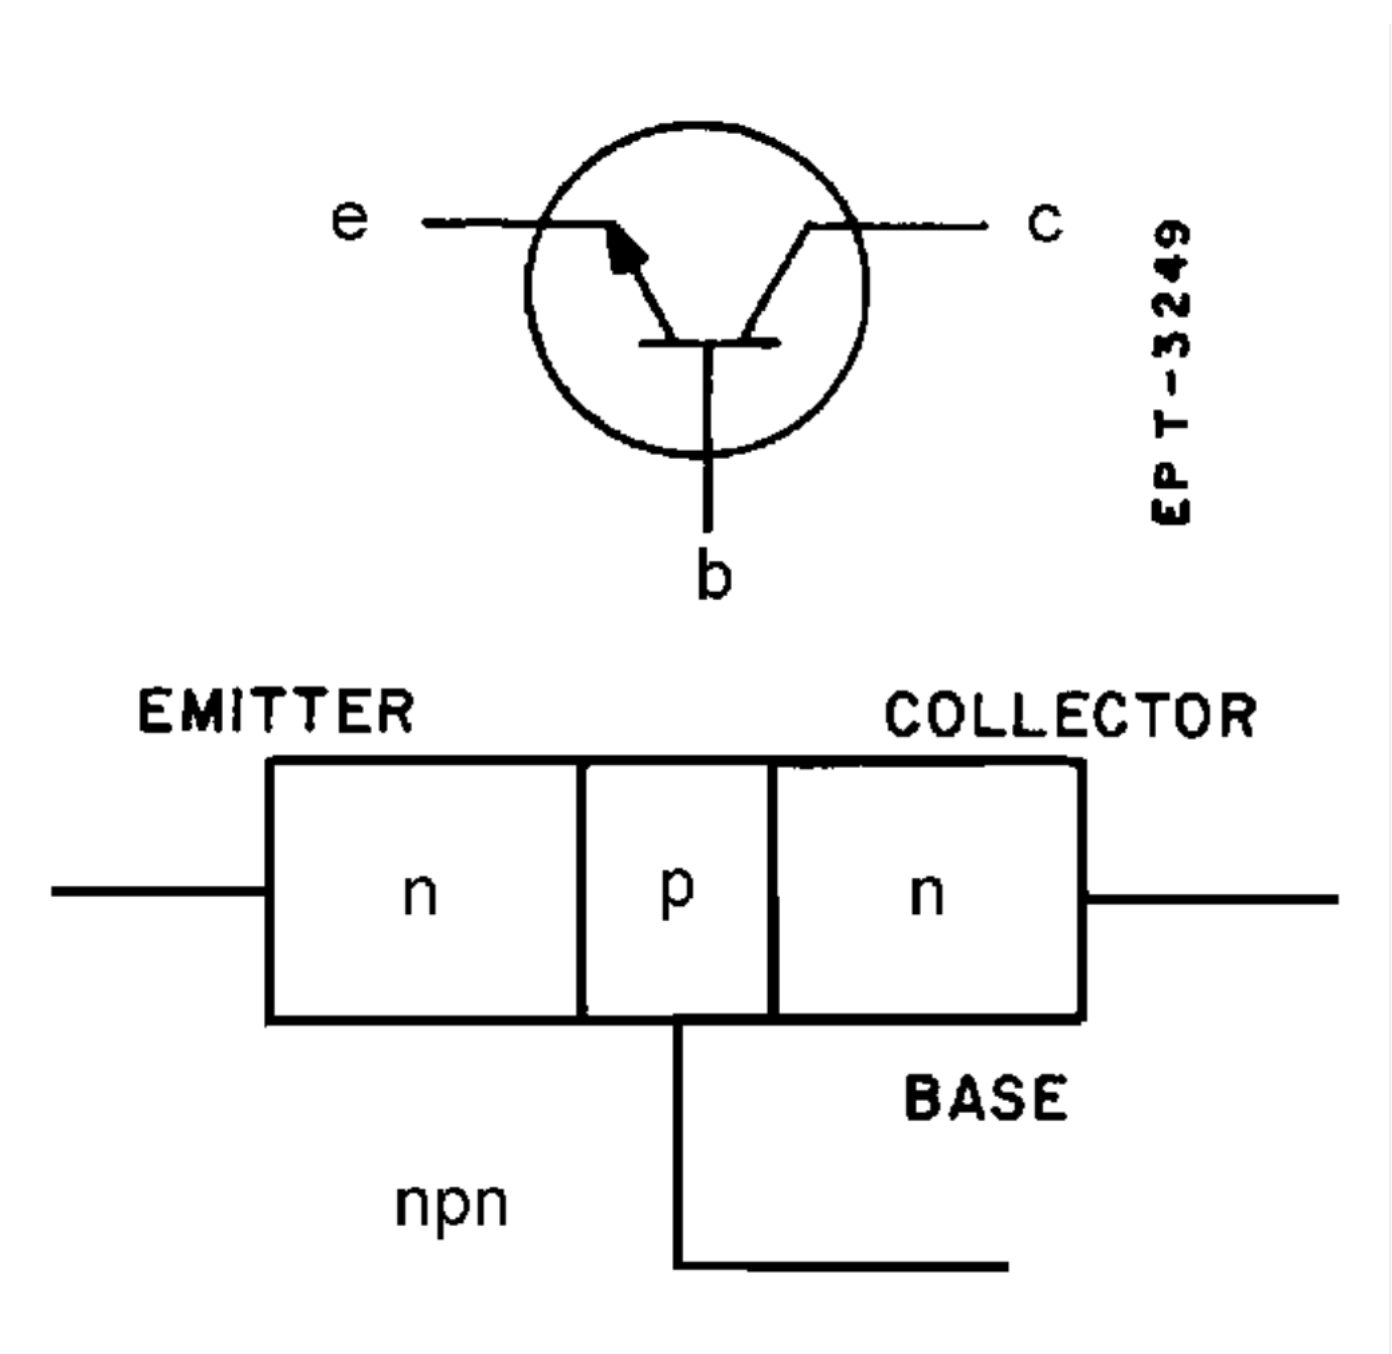
\includegraphics[scale=0.3]{NPN}}
		\captionof{figure}{The NPN Transistor}
	\end{figure}
\end{examp}
\subsubsection*{Why the 7405?}
All of this hand waving still doesn't answer the question as the difference hasn't been hammered home quite yet.

\textbf{Example 2} shows the schematics from the official Texas Instrument's Datasheets and walks through the operation. When focusing on the output \(Y\), the difference between the circuits is clear.
The 7405 chip's output BJT's collector terminal is left unconnected within the chip. This is also known as an ``open." This architecture allows the chip to be independent of the downstream current draw.

This makes it suitable for applications where a resistive load such as a motor, or in this case, an LED is connected to the output of the inverter.
This does require some planning as the load requires a external pullup resistor in order to achieve a HIGH output.

There are three possible different configurations of a BJT circuit, a common emitter, common base, or a \textit{common collector circuit} where ``Common" references which two leads of the BJT are both part of the input and outputs circuits.

For the 7405, a positive-going input signal drives the base more positive with respect to the emitter, which causes the base current to increase. This results in more emitter current, causing a more positive output voltage at the emitter to drive our LED.
\begin{examp}
	\textbf{Operation of the 7405}
	\begin{figure}[h]
		\subfigure[The Standard 7404]{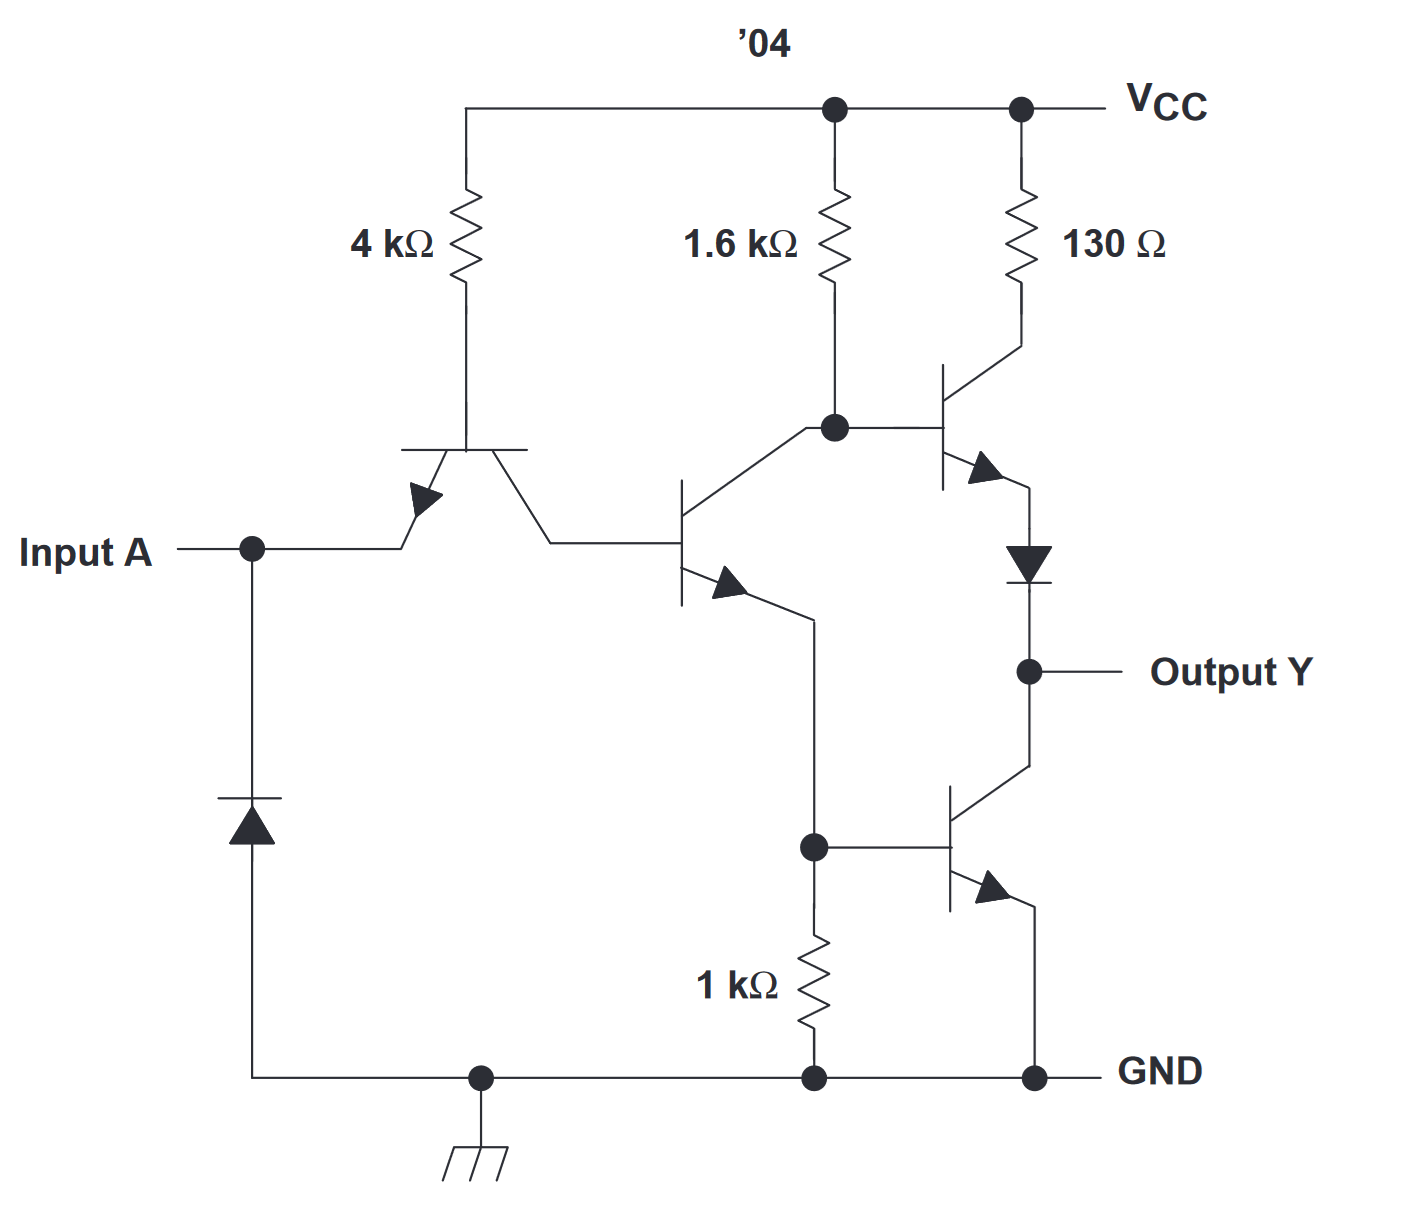
\includegraphics[width=8cm]{04}}
		\hfill
		\subfigure[The Standard 7405]{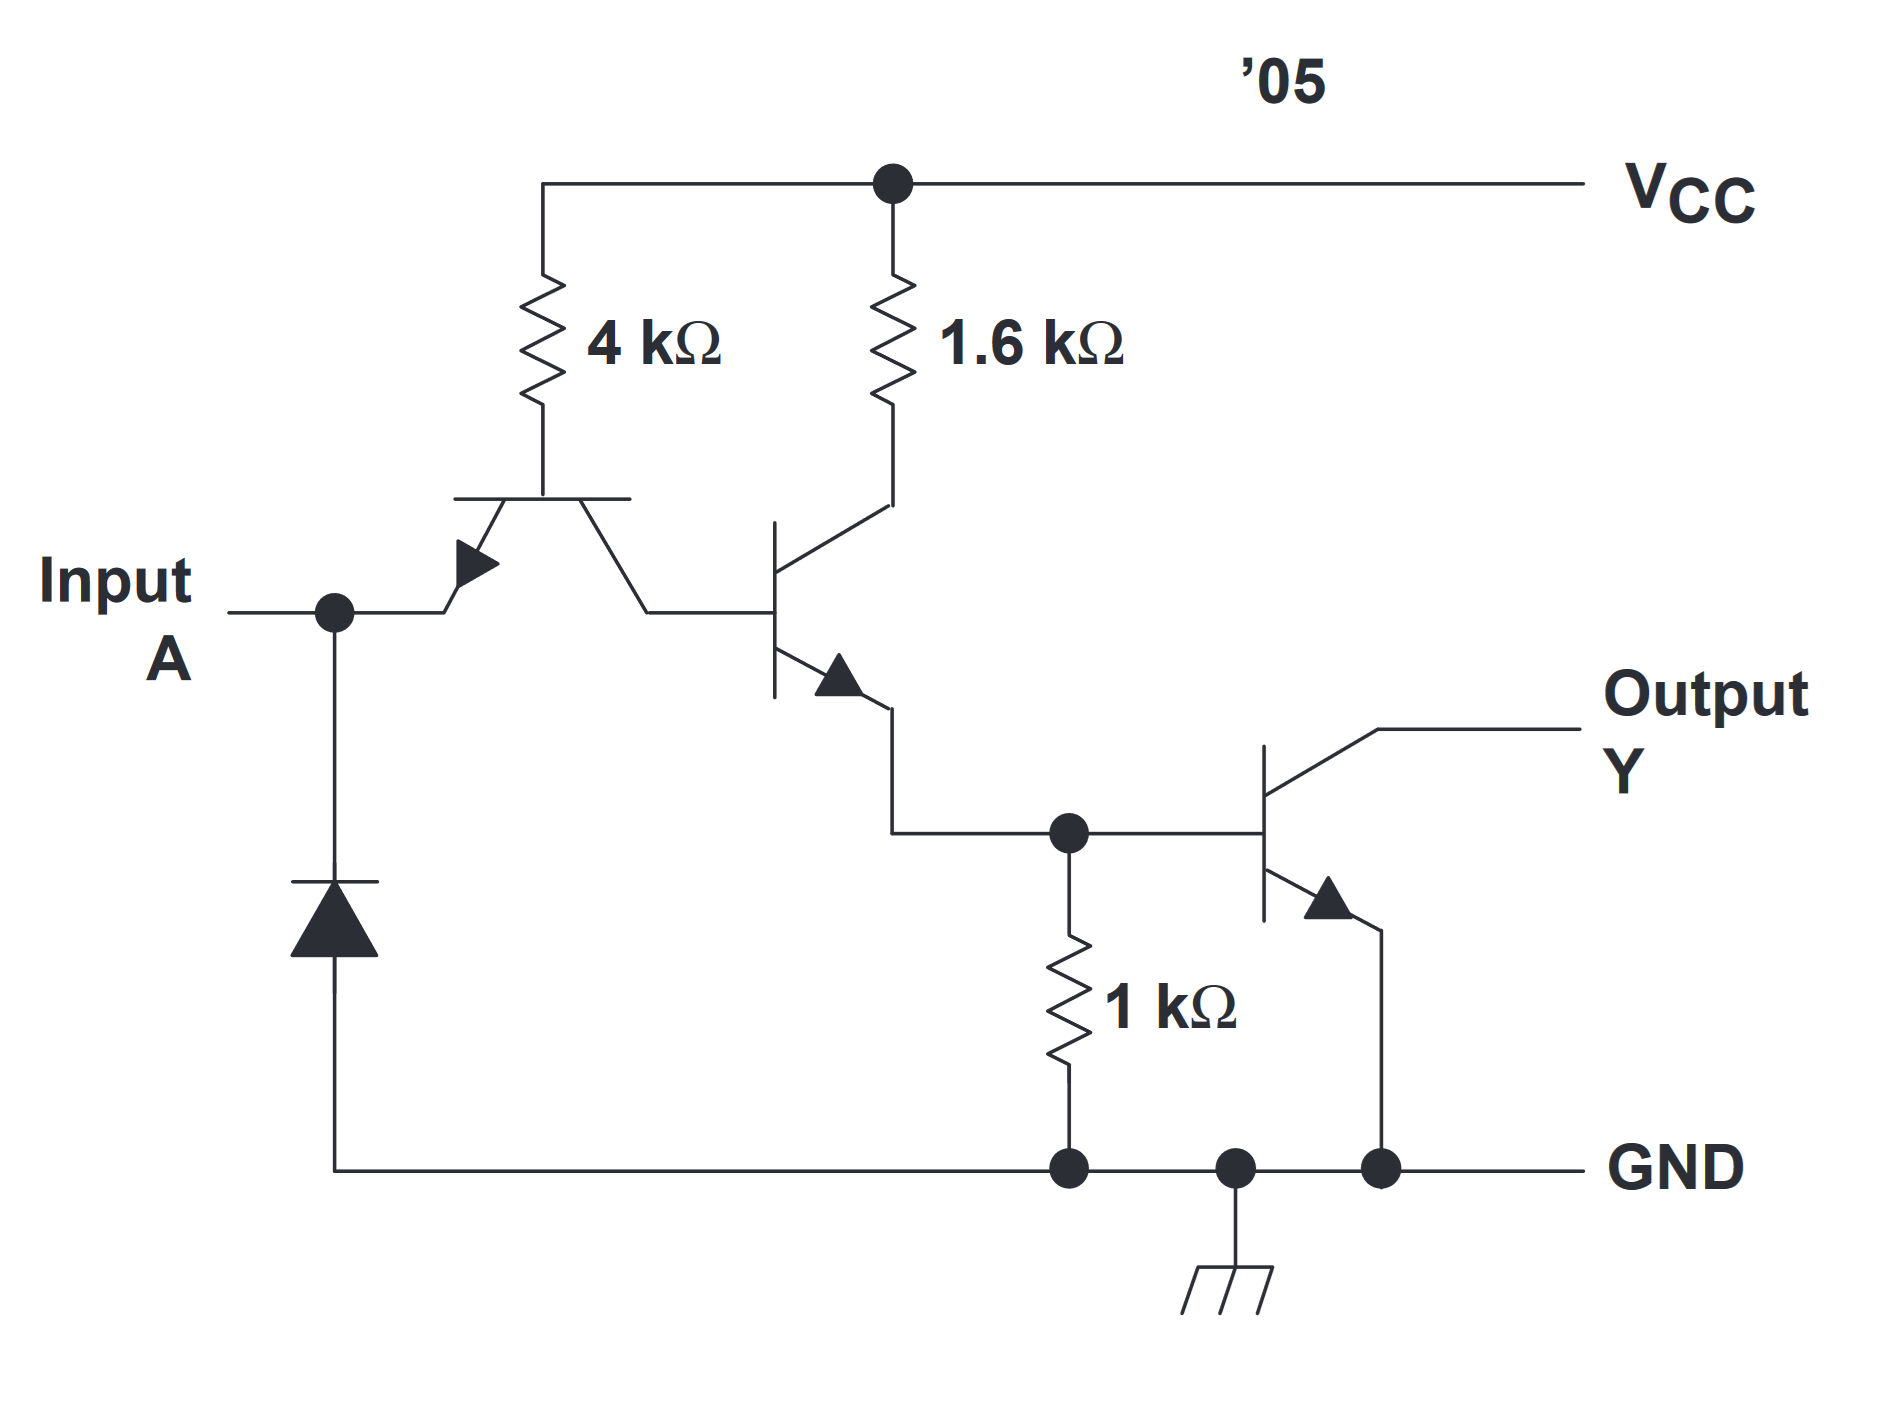
\includegraphics[width=8cm]{05}}
		\captionof{figure}{Schematic View}
	\end{figure}
	\newline
	\textnormal{When the input signal is high:}
	\begin{itemize}

		\item The base of the first NPN transistor is forward biased relative to its emitter, allowing base current to flow. This results in current flowing from the collector to the emitter, effectively grounding the output.
		\item The base current enables a larger current flow from the collector to the emitter, pulling the output low (close to ground).
		\item In this state, the transistor is ``on," and the output is a logic LOW signal (approximately 0.0V to 0.8V in TTL logic).
	\end{itemize}
	\pagebreak
	\textnormal{When the input signal is low:}
	\begin{itemize}
		\item The base of the first NPN transistor is not forward biased, so no current flows through the base-emitter junction. As a result, the collector-emitter path remains open, and the transistor is turned off.
		\item Since the transistor is off, the output floats and is pulled high by the external pull-up resistor, resulting in a logic HIGH output close to \(V_{CC}\).
	\end{itemize}
\end{examp}
In the 7405 open-collector configuration, the NPN transistor plays a crucial role in determining the output state based on the input signal.

As with any NPN transistor, the emitter, base, and collector function to control the current flow between the collector and emitter through the base current.

In this circuit, the NPN transistor's collector is left unconnected internally (hence the term ``open collector"). The external load, such as an LED or a resistive element, is connected between the output (collector) and a pull-up resistor, which is tied to the supply voltage

In essence, the NPN transistor in the 7405 circuit acts as a switch that controls the flow of current to the output based on the base current. When there is base current, the transistor conducts, and the output is pulled low. When there is no base current, the transistor is off, and the output is pulled high by the external resistor.

This open-collector design is particularly useful for applications that require the driving of higher-current loads, such as LEDs, without requiring the IC itself to supply the current. Instead, the external load provides the necessary current, allowing the circuit to handle higher loads more efficiently.

To summarize, in plain non-electrical engineering speak, if the transistor is ON, current flows through the path of least resistance and robs the output (our LED) of its current, making the light go dim. If the transistor is OFF, the pullup resistor now makes the path of least resistance between the LED and ground and the LED illuminates.
\subsection*{Current Draw of Each LED} \
The current through each LED is calculated using Ohm's Law:
\begin{examp}
	\[
		I = \frac{V_{R}}{R} = \frac{V_{\text{supply}} - V_{\text{LED}}}{R}
	\]

	Where:
	\begin{itemize}
		\item \( V_{\text{supply}} = 5V \) is the supply voltage.
		\item \( V_{\text{LED}} \) is the forward voltage of the LED.
		      This is measured at \(1.786V\) by my multimeter.
		\item \( R = 330 \, \Omega \) is the resistor value.
	\end{itemize}
	\[
		I_{\text{red}} = \frac{5V - 1.786V}{330 \, \Omega} = \frac{3.214V}{330 \, \Omega} = 9.74 \, \text{mA}
	\]
\end{examp}
\pagebreak
\section*{Deliverables}
\subsection*{POSTNET to \(\bm{XS_{3}}\) Encoding}
\begin{table}[h!]
	\centering
	\begin{tabular}{|c|c c c c c|c c c c|}
		\hline
		Decimal & V & W & X & Y & Z & D & C & B & A \\
		\hline
		0       & 1 & 1 & 0 & 0 & 0 & 0 & 0 & 1 & 1 \\
		1       & 0 & 0 & 0 & 1 & 1 & 0 & 1 & 0 & 0 \\
		2       & 0 & 0 & 1 & 0 & 1 & 0 & 1 & 0 & 1 \\
		3       & 0 & 0 & 1 & 1 & 0 & 0 & 1 & 1 & 0 \\
		4       & 0 & 1 & 0 & 0 & 1 & 0 & 1 & 1 & 1 \\
		5       & 0 & 1 & 0 & 1 & 0 & 1 & 0 & 0 & 0 \\
		6       & 0 & 1 & 1 & 0 & 0 & 1 & 0 & 0 & 1 \\
		7       & 1 & 0 & 0 & 0 & 1 & 1 & 0 & 1 & 0 \\
		8       & 1 & 0 & 0 & 1 & 0 & 1 & 0 & 1 & 1 \\
		9       & 1 & 0 & 1 & 0 & 0 & 1 & 1 & 0 & 0 \\
		\hline
	\end{tabular}
	\caption{POSTNET to XS3 Conversion Table}
\end{table}
From here, each output signal \(D, C, B, A\) is isolated into its own, separate equation, signifying the combination of inputs necessary to eventually output a 4-bit \(XS_{3}\) encoded output.
\begin{examp}
\textbf{D Output}

The map is divided into two layers for $V=0$ and $V=1$. Pay Attention to $V$.
\begin{center}
\begin{karnaugh-map}(label=corner)[4][4][2][$Z$][$Y$][$X$][$W$][$V$]
\minterms{10,12,17,18,10}
\maxterms{3,5,6,8,24}
\autoterms[X]
\implicant{12}{14}[0]
\implicant{15}{10}[0]
\implicant{0}{6}[1]
\end{karnaugh-map}
\end{center}

This produces:
\[
	D = \closure{V}(WX + WY) + V(\closure{W})
\]
\[
	D = \closure{V}WX + \closure{V}WY + V\closure{W} \quad \text{(Distribution)}
\]
\[
	D =  WX + WY + V\closure{W} \quad \text{(Absorption)}
\]
\end{examp}
\newpage
\begin{examp}
\textbf{C Output}
\begin{center}
\begin{karnaugh-map}(label=corner)[4][4][2][$Z$][$Y$][$X$][$W$][$V$]
\minterms{4,19,21,22,25}
\maxterms{1,2,8,28,26}
\autoterms[X]
\implicant{4}{14}[0]
\implicantedge{0}{1}{8}{9}[1]
\implicant{0}{6}[1]
\end{karnaugh-map}
\end{center}

This produces:
\[
	C = \closure{V}(\closure{W} + \closure{X}Y) + V(X)
\]
\[
	C = \closure{V}\closure{W} + \closure{V}\closure{X}Y + VX \quad \text{(Distribution)}
\]
\end{examp}

\begin{examp}
\textbf{B Output}
\begin{center}
\begin{karnaugh-map}(label=corner)[4][4][2][$Z$][$Y$][$X$][$W$][$V$]
\minterms{6,9,17,18,24}
\maxterms{20,3,5,12,10}
\autoterms[X]
\implicant{1}{11}[1]
\implicantcorner[1]
\implicantedge{0}{1}{8}{9}[0]
\implicant{7}{14}[0]
\end{karnaugh-map}
\end{center}

This produces:
\[
	B = \closure{V}(\closure{X}\closure{Y} + XY) + V(\closure{X}\closure{Z} + Z)
\]
\[
	B = \closure{V}(\closure{X}\closure{Y} + XY) + V(\closure{X} + Z) \quad \text{(Absorption)}
\]
\[
	B = \closure{V}\closure{X}\closure{Y} + \closure{V}XY + V\closure{X} + VZ \quad \text{(Distribution)}
\]
\end{examp}
\newpage
\begin{examp}
\textbf{A Output}
\begin{center}
\begin{karnaugh-map}(label=corner)[4][4][2][$Z$][$Y$][$X$][$W$][$V$]
\minterms{5,12,9,18,24}
\maxterms{20,17,3,6,10}
\autoterms[X]
\implicant{0}{9}[0]
\implicantedge{0}{0}{2}{2}[1]
\implicant{12}{10}[1]
\end{karnaugh-map}
\end{center}
This produces:
\[
	A = \closure{V}\closure{Y} + V(\closure{W}\closure{X}\closure{Z} + W)
\]
\[
	A = \closure{V}\closure{Y} + V\closure{W}\closure{X}\closure{Z} + VW \quad \text{(Distribution)}
\]
\end{examp}
\section*{Discussion}
Ultimately, this lab aided me in gaining experience with Karnaugh maps and reducing boolean expressions. The 3D representation of the K-maps in the documentation allowed for a simpler visualization of this in my own head. It was actually quite engaging and took a lot of carful attention to detail to each and every single value. I found myself having multiple transcription errors, but in doing this, I gained a lot more practice.

The introduction to the breadboard and having hands on real hardware was a nice change in pace for me. I have not worked with physical hardware since I was attached to Reactor Controls division on a nuclear fast attack submarine. Nevertheless, it was interesting to see how much more lenient the lab can be when only dealing with 5V coming from the transformers compared to the vast hoops I had to jump through with electrical safety in the Nuclear Navy.

Careful attention was placed on cable routing as this is paramount to allow for comprehensive troubleshooting down the line. Looking forward to the other labs, I want to learn more complex combinational logic and start gronking the sequential logic again that I was exposed to in Nuclear Field Electronics Technician 'A' School many years ago. The pace and military obligations during `A` school were way too demanding to appreciate the subject and what it is that we learned, it was just a fire hose of information for 2 years straight 7am to frequently close to 8pm. The slower pace of a University course where more attention is given to everyone is a breath of fresh air as it allows me to really get into the weeds of what the specifics are. For this lab, I reviewed silicon doping and how a PN Junction works in order to understand (or better yet, remember) how a BJT's components react to different values of potential.

This sparked a lot of memories of troubleshooting various circuit cards on the boat and reading endless documentation until the problem was identified and the guilty components replaced, installed, and retested. It also allowed for use of some standardized lab equipment such as a digital multimeter and a logic probe, which I am very excited to continue working with.
% Practice Questions Section
\section*{Practice Questions}
\begin{examp}
\vspace{3mm}
\textbf{Karnaugh Map for \(\bm{\sum m(0, 2, 3, 4, 6, 7, 8, 10, 12)}\)}
\begin{center}
\begin{karnaugh-map}(label=corner)[4][4][1][$D$][$C$][$B$][$A$]
\minterms{0,2,3,4,6,7,8,10,12}
\autoterms[0]
\implicantcorner
\implicant{3}{6}
\implicant{0}{8}
\end{karnaugh-map}
\end{center}
\textit{This produces:}
\[
	F(A,B,C,D) = \closure{A}C + \closure{B}\closure{D} + \closure{C}\closure{D}
\]
\[
	F(A,B,C,D) = \closure{A}C + \closure{D}(\closure{B} + \closure{C}) \quad \text{\textit{(Distribution)}}
\]
\end{examp}
\begin{examp}
	\vspace{3mm}
	\textbf{IEEE-754 Floating Point Conversion}
	\newline
	We are tasked with converting $-19.5_{10}$ into Single Precision IEEE-754 floating point format. We will show the sign bit, exponent, and first 8-bits of the mantissa.

	\textbf{Step 1: Determine the sign bit $\bm{(S)}$}

	Since the number is negative, the sign bit is:
	\[
		S = 1	\]

	\textbf{Step 2: Convert the magnitude \(\bm{19.5_{10}}\) to binary}

	First, we convert the integer part and the fractional part of \(19.5_{10}\) to binary:
	\[
		19_{10} = 10011_2 \quad \text{and} \quad 0.5_{10} = 0.1_2
	\]
	Therefore, the binary representation of \(19.5_{10}\) is:
	\[
		10011.1_2\]

	\textbf{Step 3: Normalize the binary number}

	We normalize $10011.1_2$ into the form $1.M \times 2^E$ by shifting the decimal point 4 places to the left:
	\[
		10011.1_2 = 1.00111_2 \times 2^4
	\]

	Here, the mantissa $M$ is $00111_2$, and the exponent $E$ is $4$.

	\textbf{Step 4: Calculate the biased exponent}

	The exponent is biased by 127 in Single Precision IEEE-754. So, we add 127 to the actual exponent $4$:
	\[
		E = 127 + 4 = 131
	\]
	Converting to binary, we get:
	\[
		E = 10000011_2
	\]

	\textbf{Step 5: Assemble the IEEE-754 representation} \\
	Now we can assemble the components:
	\begin{itemize}
		\item Sign bit $S = 1$
		\item Exponent $E = 10000011_2$
		\item Mantissa $M = 00111_2$ (we add trailing zeros to get the first 8 bits: $00111000_2$)
	\end{itemize}
	Thus, the first 17 bits of the IEEE-754 floating-point representation of $-19.5_{10}$ are:
	\[
        1 \ 10000011 \ 00111000_{IEEE-754}
	\]

	\textbf{Final Answer:}
	The IEEE-754 single-precision representation of $-19.5_{10}$ (with the first 8 bits of the mantissa) is:
	\[
        1 \ 10000011 \ 00111000_{IEEE-754}
	\]
\end{examp}
\end{document}
% vim: set spell spelllang=en_us expandtab tabstop=4 shiftwidth=4 softtabstop=4:
